\documentclass[10pt]{beamer}
\usetheme[
%%% option passed to the outer theme
%    progressstyle=fixedCircCnt,   % fixedCircCnt, movingCircCnt (moving is deault)
  ]{Feather}
  
% If you want to change the colors of the various elements in the theme, edit and uncomment the following lines

% Change the bar colors:
\setbeamercolor{Feather}{fg=shtred!20,bg=shtred}

% Change the color of the structural elements:
\setbeamercolor{structure}{fg=shtred}

% Change the frame title text color:
%\setbeamercolor{frametitle}{fg=blue}

% Change the normal text color background:
%\setbeamercolor{normal text}{fg=black,bg=gray!10}

%-------------------------------------------------------
% INCLUDE PACKAGES
%-------------------------------------------------------

\usepackage[utf8]{inputenc}
\usepackage[english]{babel}
\usepackage[T1]{fontenc}
\usepackage{helvet}
\usepackage{subcaption}
\usepackage{amsmath}

\makeatletter
\renewcommand*\env@matrix[1][*\c@MaxMatrixCols c]{%
  \hskip -\arraycolsep
  \let\@ifnextchar\new@ifnextchar
  \array{#1}}
\makeatother
%-------------------------------------------------------
% DEFFINING AND REDEFINING COMMANDS
%-------------------------------------------------------

% colored hyperlinks
\newcommand{\chref}[2]{
  \href{#1}{{\usebeamercolor[bg]{Feather}#2}}
}

%-------------------------------------------------------
% INFORMATION IN THE TITLE PAGE
%-------------------------------------------------------

\title[] % [] is optional - is placed on the bottom of the sidebar on every slide
{ % is placed on the title page
      \textbf{Linear Algebra - Introduction}
}

\subtitle[ Linear Algebra - Introduction ]
{
      \textbf{}
}

\author[Lovish]
{      Lovish \\
	lovish1234@gmail.com
}

\institute[]
{
      Center for Visual Information Technology\\
    IIIT Hyderabad\\
  
  %there must be an empty line above this line - otherwise some unwanted space is added between the university and the country (I do not know why;( )
}

\date{June 4, 2018}

%-------------------------------------------------------
% THE BODY OF THE PRESENTATION
%-------------------------------------------------------

\begin{document}

%-------------------------------------------------------
% THE TITLEPAGE
%-------------------------------------------------------

{\1% % this is the name of the PDF file for the background
\begin{frame}[plain,noframenumbering] % the plain option removes the header from the title page, noframenumbering removes the numbering of this frame only
  \titlepage % call the title page information from above
\end{frame}}


\begin{frame}{Contents}{}
\tableofcontents
\end{frame}

%-------------------------------------------------------
\section{Trivia}
%-------------------------------------------------------
\subsection{Motivation}
\begin{frame}{Trivia}{Motivation}
%-------------------------------------------------------
  \begin{itemize}
    \item As machine learning practitioners, it is important to understand underlying operations in libraries such as \textit{numpy, torch}
    \pause
    \begin{itemize}
    \item Almost all of these libraries act on objects called \textit{matrices} or \textit{tensors}
    \pause
    \item Why ? Majority of data that these libraries act upon such as time series, language or images can be represented as these objects
    \end{itemize}
    \pause
    \item As life long learners, we should understand the abstract concept of algebraic structures called \textbf{vector spaces}
    \pause
    \begin{itemize}
    \item A very naive application is solving a linear system of equations 
    \pause
    \item ??
    \end{itemize}
  \end{itemize}
\end{frame}



\subsection{Charter}
\begin{frame}{Trivia}{Charter}
%-------------------------------------------------------
  \begin{itemize}
    \item Learn linear algebra to be comfortable with Machine Learning
    \begin{itemize}
    \item How can we perform matrix computations with \textbf{acceptable speed and accuracy} ?
    \item What is the role of \textbf{numerical stability} in this regard ?
    \end{itemize}
    \item Learn through visualization and examples
    \item Broach upon abstractions which we sometimes encounter in technical papers

  \end{itemize}
\end{frame}

\subsection{Acknowledgements}
\begin{frame}{Trivia}{Acknowledgements}
%-------------------------------------------------------
  \begin{itemize}
    \item Linear Algebra by Gilbert Strang \href{https://ocw.mit.edu/courses/mathematics/18-06-linear-algebra-spring-2010/video-lectures/}{\beamergotobutton{Link}}
    \item \alert{Essence of Linear Algebra by Grand Sanderson} \href{https://www.youtube.com/watch?v=kjBOesZCoqc&list=PLZHQObOWTQDPD3MizzM2xVFitgF8hE_ab}{\beamergotobutton{Link}}
    \item Computational Linear Algebra by Fast.ai \href{http://www.fast.ai/2017/07/17/num-lin-alg/}{\beamergotobutton{Link}}
    \item Immersive Linear Algebra by J. Storm et al      \href{http://immersivemath.com/ila/index.html}{\beamergotobutton{Link}}


  \end{itemize}
\end{frame}

\subsection{Conventions}
\begin{frame}{Trivia}{Conventions}
%-------------------------------------------------------
  \begin{itemize}
    \item scalars are written in lowecase and \textit{italics}.
    \item vectors are written in lowercase and \textbf{bold}
    \item Matrices are written in Uppercase and \textbf{bold}
  \end{itemize}
\end{frame}



\subsection{Miscellaneous}
\begin{frame}{Trivia}{Miscellaneous}
%-------------------------------------------------------
  \begin{itemize}
  \item Lecture 1 - Solving a system of linear equations
  \begin{itemize}
  \item Particular Solution
  \item General Solutions
  \end{itemize}
  \item Lecture 2 - Abstract vector spaces 
  \item Lecture 3 - Matrix Decomposition based on solving system of linear equations  
  \begin{itemize}
  \item LU
  \item QR
  \end{itemize}
  \item Lecture 4 - Matrix Decomposition based on eigendecomposition 
  \begin{itemize}
  \item Eigen Value Decomposition
  \item Singular Value Decomposition
  \end{itemize}
  \item Lecture 5 - Computational Issues
  \item Lecture 6 - \textit{Omakase} Lecture
  \end{itemize}
\end{frame}




%-------------------------------------------------------
\section{Introduction}
%-------------------------------------------------------
\subsection{Vectors}
\begin{frame}{Introduction}{Vectors}

%-------------------------------------------------------
\begin{itemize}
\item \textbf{High School} - A vector is a scalar which also happens to have a direction. eg. $ \hspace{0.1in} \vec{f} = m.\vec{a} $
\item \textbf{University Sophomore} - An abstract concepts, an entity that resides in a vector space. It follows these two rules :-
\begin{itemize}
\item It can be added together with another object to get an object of same kind
\item It can be multiplied with a scalar and the resultant object is of the same kind
\end{itemize}
\item \textbf{Big Data Engineer} - It is a list of real numbers $\mathbb{R}^{n}$
\end{itemize}

\begin{figure}[!htb]
\centering
\begin{subfigure}[t]{0.30\linewidth}
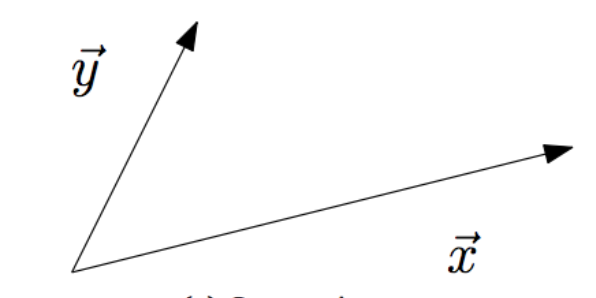
\includegraphics[width=0.90\textwidth]{Feathergraphics/school.png}
\caption{High School}
\end{subfigure}
\begin{subfigure}[t]{0.30\linewidth}
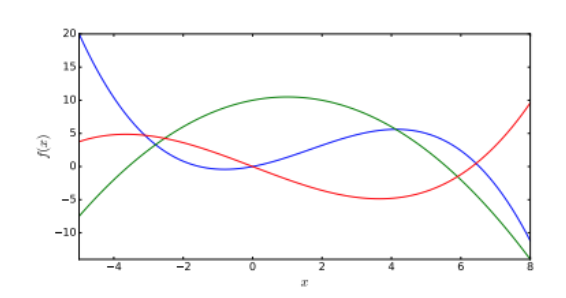
\includegraphics[width=0.90\textwidth]{Feathergraphics/univ.png}
\caption{University}
\end{subfigure}
\begin{subfigure}[t]{0.30\linewidth}
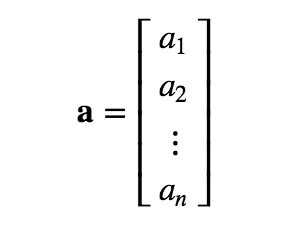
\includegraphics[width=0.90\textwidth]{Feathergraphics/eng.png}
\caption{Data Science Engineer}
\end{subfigure}

\vspace{0.1in}
\label{fig:tripEmb}
\end{figure}

\end{frame}


\subsection{Linear Equations}
\begin{frame}{Introduction}{Linear Equations}

%-------------------------------------------------------
\begin{itemize}
\item Why should we learn to solve a linear equation ?
\pause
\begin{itemize}
\item Determine if set of vectors are \textbf{linearly independent}
\item Determine the \textbf{rank} of the matrix 
\item Determine the \textbf{basis} of vector space
\item Solving $\textbf{A}\textbf{x} = \textbf{b}$
\end{itemize}

\item Today's Content

\begin{itemize}
\item Particular and General Solutions of linear equation
\item Row Echelon and Reduced row echelon form
\item Gaussian Elimination
\end{itemize}


\end{itemize}
\end{frame}
%--------------------------------------------
\begin{frame}{Introduction}{Linear Equation}

A set of equations can have unique solution, no solution or infinitely many solutions.

Set 1 
$$ x_{1} + x_{2} + x_{3} = 3  $$
$$ x_{1} - x_{2} + 2x_{3} = 2 $$
$$ 2x_{1} + 3x_{3} = 1 $$

Set 2
$$ x_{1} + x_{2} + x_{3} = 3  $$
$$ x_{1} - x_{2} + 2x_{3} = 2 $$
$$ x_{2} + x_{3} = 2 $$

Set 3
$$ x_{1} + x_{2} + x_{3} = 3  $$
$$ x_{1} - 2x_{2} + x_{3} = 2 $$
$$ 2x_{1} + 3x_{3} = 5 $$

\end{frame}


%--------------------------------------------
\begin{frame}[shrink=20]{Introduction}{Linear Equation}

Let us change the way we write the above equations

\begin{align}
x_{1}\begin{bmatrix}1 \\ 1 \\ 2 \end{bmatrix} + x_{2}\begin{bmatrix} 1 \\ -1 \\ 0 \end{bmatrix} + x_{3}\begin{bmatrix}1 \\ 2 \\ 3 \end{bmatrix} = \begin{bmatrix} 3 \\ 2 \\ 1 \end{bmatrix} \Leftrightarrow \begin{bmatrix} 1 & 1 & -1 \\ 1 & -1 & 2 \\ 2 & 0 & 3 \end{bmatrix}\begin{bmatrix} x_{1} \\ x_{2} \\ x_{3}\end{bmatrix} = \begin{bmatrix} 3 \\ 2 \\ 1 \end{bmatrix}
\end{align}


\begin{align}
x_{1}\begin{bmatrix}a_{11}\\\vdots\\a_{m1}\end{bmatrix}+x_{2}\begin{bmatrix}a_{12}\\\vdots\\a_{m2}\end{bmatrix}+\cdots+x_{n}\begin{bmatrix}a_{1n}\\\vdots\\a_{mn}\end{bmatrix} = \begin{bmatrix}b_{1}\\\vdots\\b_{m}\end{bmatrix} \Leftrightarrow   \begin{bmatrix} a_{11} & \cdots & a_{1n}\\ \vdots & \vdots & \vdots \\ a_{m1} & \cdots & a_{mn}\end{bmatrix} \begin{bmatrix} x_{1}\\ \vdots \\ x_{n}\end{bmatrix}=\begin{bmatrix} b_{1}\\ \vdots \\ b_{n}\end{bmatrix}
\end{align}

On the right side is something we call the compact representation of linear system of equations. We can write it as :-

$$ \textbf{A}\textbf{x} = \textbf{b}$$

Note that this representation multiplies columns of the matrix with the individual entries in vector $\textbf{x}$.

\end{frame}



%--------------------------------------------
\subsection{Particular Solution}
\begin{frame}{Introduction}{Particular Solution}

Find \textbf{single solution} to the following equation :- 
\begin{align}
\begin{bmatrix} 1 & 0 & 8 & -4 \\ 0 & 1 & 2 & 12 \end{bmatrix}\begin{bmatrix}x_{1}\\x_{2}\\x_{3}\\x_{4}\end{bmatrix} = \begin{bmatrix}42\\8\end{bmatrix}
\end{align}

\pause 
\begin{itemize}
\item $$ \sum_{i=1}^{4}x_{i}\textbf{c}_{i} = \textbf{b}$$ where $\textbf{c}_{i}$ are the columns of $\textbf{A}$
\pause
\item Look at the first two columns of the matrix
\end{itemize}



\end{frame}

\subsection{General Solutions}
\begin{frame}{Introduction}{General Solutions}

But what do we need to find \textbf{all} the solutions :- 
\begin{align}
\begin{bmatrix} 1 & 0 & 8 & -4 \\ 0 & 1 & 2 & 12 \end{bmatrix}\begin{bmatrix}x_{1}\\x_{2}\\x_{3}\\x_{4}\end{bmatrix} = \begin{bmatrix}42\\8\end{bmatrix}
\end{align}
\pause
 
\begin{itemize}
\item Find the solutions to $\textbf{A}\textbf{x}= \textbf{0}$
\pause
\item Is there a way we can represent rest of the columns as sum of first two columns
\end{itemize}
\end{frame}

%----------------------------------------------------

\begin{frame}{Introduction}{General Solutions}

Is there a way we can represent the third column as sum of first two columns
\begin{align}
\begin{bmatrix} 1 & 0 & 8 & -4 \\ 0 & 1 & 2 & 12 \end{bmatrix} \begin{pmatrix} \lambda_{1}\begin{bmatrix}?\\?\\?\\0\end{bmatrix} \end{pmatrix}= \begin{bmatrix}0\\0\end{bmatrix}
\end{align}

What about fourth column ?

\pause 

\begin{align}
\begin{bmatrix} 1 & 0 & 8 & -4 \\ 0 & 1 & 2 & 12 \end{bmatrix} \begin{pmatrix} \lambda_{1}\begin{bmatrix}?\\?\\0\\?\end{bmatrix} \end{pmatrix}= \begin{bmatrix}0\\0\end{bmatrix}
\end{align}

\end{frame}


%----------------------------------------------------

\begin{frame}{Introduction}{General Solutions}

Finally, putting everything together, we obtain a general solution to the linear system of equations which we call \textbf{general solution}.

\begin{align}
x=\begin{bmatrix}42\\8\\0\\0\end{bmatrix} + \begin{pmatrix} \lambda_{1}\begin{bmatrix}8\\2\\-1\\0\end{bmatrix} \end{pmatrix} + \begin{pmatrix} \lambda_{1}\begin{bmatrix}-4\\12\\0\\-1\end{bmatrix} \end{pmatrix}, \lambda_{1},\lambda_{2} \in \mathbb{R}
\end{align}

\begin{itemize}
\item But how about any other equation ? Can it be solved the same way.
\end{itemize}

\end{frame}


%----------------------------------------------------

\begin{frame}{Introduction}{General Solutions}

Steps for finding the general solution of a equation :-

\begin{itemize}
\item  Find a particular solution to $\textbf{A}\textbf{x}=\textbf{b}$
\item Find all solutions to $\textbf{A}\textbf{x}=\textbf{0}$
\item Combine step 1 and 2 to get a general solution
\end{itemize}

\pause 

Suppose that the equation is :-

\begin{align}
\begin{bmatrix} \alert{5} & \alert{-27} & 8 & -4 \\ \alert{7} & \alert{19} & 2 & 12 \end{bmatrix}\begin{bmatrix}x_{1}\\x_{2}\\x_{3}\\x_{4}\end{bmatrix} = \begin{bmatrix}42\\8\end{bmatrix}
\end{align}

\pause 

We have to convert the above equation to \textit{convenient form} as the Equation (3).
\end{frame}

\subsection{Gauss Elimination}
\begin{frame}[shrink=20]{Introduction}{Gauss Elimination}

\vspace{0.25in}

We would like to keep the solution set the same while transforming the set of equations into this \textit{convenient form}. Take the following set of equations :-

$$ -2x_{1} + 4x_{2} - 2x_{3} - x_{4} + 4x_{5} = -3 $$
$$ 4x_{1} - 8x_{2} + 3x_{3} - 3x_{4} + x_{5} = 2 $$
$$ x_{1} - 2x_{2} + x_{3} - x_{4} + x_{5} = 0 $$
$$ x_{1} - 2x_{2} - 3x_{4} + 4x_{5} = a$$

We can write it as :-

\begin{align}
\begin{bmatrix} -2 & 4 & -2 & -1 & 4 \\ 4 & -8 & 3 & -3 & 1 \\ 1 & -2 & 1 & -1 & 1 \\ 1 & -2 & -3 & 0 & 4 \end{bmatrix}\begin{bmatrix} x_{1} \\ x_{2} \\ x_{3} \\ x_{4} \\ x_{5}\end{bmatrix} = \begin{bmatrix}-3 \\ 2 \\ 0 \\ a \end{bmatrix} \Leftrightarrow   \begin{bmatrix}[ccccc|c]
   -2 & 4 & -2 & -1 & 4 & -3 \\
   4 & -8 & 3 & -3 & 1 & 2\\
   1 & -2 & 1 & -1 & 1 & 0\\
   1 & -2 & -3 & 0 & 4 & a
\end{bmatrix}
\end{align}

What should be those transforms ? 

\end{frame}

\begin{frame}{Introduction}{Gauss Elimination}

\begin{block}{Elemetary Transformations}
\begin{itemize}
\item Exchange of two equations (or row in the matrix representing the equation system)
\item Multiplication of an equation with a constant $\lambda \in \mathbb{R} \setminus \{0\}$
\item Addition of an equation(row) to another equation(row)
\end{itemize}
\end{block}


\begin{block}{Row Echelon Form}
\begin{itemize}
\item The leading coefficient of nonzero row is always strictly to the right of the leading coefficient of the row above it.
\item If a row contains a non-zero element at a certain column, the elements below it should all be zero.
\end{itemize}
\end{block}


\end{frame}

\begin{frame}[shrink=20]{Introduction}{Gauss Elimination}

\begin{align}
\begin{bmatrix}[ccccc|c]
   -2 & 4 & -2 & -1 & 4 & -3 \\
   4 & -8 & 3 & -3 & 1 & 2\\
   1 & -2 & 1 & -1 & 1 & 0\\
   1 & -2 & -3 & 0 & 4 & a
\end{bmatrix} \Leftrightarrow 
\begin{bmatrix}[ccccc|c]  1 & -2 & 1 & -1 & 1 &  0 \\  0 & 0 & -1 & 1 & 3 &  -2\\ 0 & 0 & 0 & 1 & -2 &  1\\ 0 & 0 & 0 & 0 & 0 &  a+1\\ \end{bmatrix}
\end{align}

Let's complete it step by step.
\begin{enumerate}

\pause
\item  Take the row with least first element to the top row. Here we exchange the first row with the third row. $R_{1} \leftrightarrow R_{3}$ 

\begin{align}
\begin{bmatrix}[ccccc|c]  1 & -2 & 1 & -1 & 1 &  0 \\  4 & -8 & 3 & -3 & 1 &  2\\ -2 & 4 & -2 & -1 & 4 &  -3\\ 1 & -2 & 0 & -3 & 4 &  a\\ \end{bmatrix}
\end{align}

\pause
\item Now we can subtract rest of the three rows by first row such that their first element becomes 0. $R_{2} \rightarrow R_{2}-4R_{1}$, $R_{3} \rightarrow R_{3}+2R_{1}$, $R_{4} \rightarrow R_{4}-R_{1}$ 

\begin{align}
\begin{bmatrix}[ccccc|c]  1 & -2 & 1 & -1 & 1 &  0 \\  0 & 0 & -1 & 1 & -3 &  2\\ 0 & 0 & 0 & -3 & 6 &  -3\\ 0 & 0 & -1 & -2 & 3 &  a\\ \end{bmatrix}
\end{align}

\end{enumerate}

\end{frame}


\begin{frame}[shrink=20]{Introduction}{Gauss Elimination}


Let's complete it step by step.

\begin{align}
\begin{bmatrix}[ccccc|c]  1 & -2 & 1 & -1 & 1 &  0 \\  0 & 0 & -1 & 1 & -3 &  2\\ 0 & 0 & 0 & -3 & 6 &  -3\\ 0 & 0 & -1 & -2 & 3 &  a\\ \end{bmatrix}
\end{align}

\begin{enumerate}
\setcounter{enumi}{2}

\pause
\item  Take the row with least first element to the top row. Here we exchange the first row with the third row. $R_{1} \leftrightarrow R_{3}$ 

\begin{equation}
\begin{bmatrix}[ccccc|c] 1 & -2 & 1 & -1 & 1 &  0 \\  0 & 0 & -1 & 1 & -3 &  2\\ 0 & 0 & 0 & -3 & 6 &  -3\\ 0 & 0 & 0 & -3 & 6 &  a-2\\ \end{bmatrix}
\end{equation}

\pause
\item  Complete rest of the reduction procedure on your own. Finally you would have the following matrix :-

\begin{equation}
\begin{bmatrix}[ccccc|c]  1 & -2 & 1 & -1 & 1 &  0 \\  0 & 0 & -1 & 1 & 3 &  -2\\ 0 & 0 & 0 & 1 & -2 &  1\\ 0 & 0 & 0 & 0 & 0 &  a+1\\ \end{bmatrix}
\end{equation}

\end{enumerate}

\end{frame}


\begin{frame}[shrink=20]{Introduction}{Gauss Elimination}

\vspace{0.25in}

Can you tell how to solve this equation in present form ?

\begin{equation}
\begin{bmatrix}[ccccc|c] \textbf{1} & -2 & 1 & -1 & 1 &  0 \\  0 & 0 & \textbf{-1} & 1 & 3 &  -2\\ 0 & 0 & 0 & \textbf{1} & -2 &  1\\ 0 & 0 & 0 & 0 & 0 &  \textbf{a+1}\\ \end{bmatrix}
\end{equation}

The above matrix is now in row echelon form. 

\begin{itemize}

\pause
\item Taking the columns with only \textbf{pivot elements}
\begin{equation}
\begin{bmatrix}  1  & 1 & -1 &  0 \\  0 & 1  & -1 &  -2\\ 0 & 0  & 1 &  1\\ 0 & 0  & 0 &  a+1\\ \end{bmatrix}
\end{equation}

\pause
\item Determine $\lambda_{i}$ such that $b=\sum_{i=1}^{P}\lambda_{i}p_{i}$ where $p_{i}$ are the pivot columns.

\begin{align}
\lambda_{1}\begin{bmatrix}1\\0\\0\\0\end{bmatrix}+\lambda_{2}\begin{bmatrix}1\\1\\0\\0\end{bmatrix}+\lambda_{3}\begin{bmatrix}-1\\-1\\1\\0\end{bmatrix} = \begin{bmatrix}0\\-2\\1\\0\end{bmatrix}
\end{align}

\end{itemize}

\end{frame}

\subsection{Gauss-Jordan Elimination}
\begin{frame}[shrink=20]{Introduction}{Gauss-Jordan Elimination}

\vspace{0.25in}

How to get a general solution to a particular equation ?

\begin{block}{Reduced Row Echelon Form}
\begin{itemize}
\item All the rules for row echelon form
\item Every pivot element must be 1
\item The pivot element must be the only non-zero entry in it's column
\end{itemize}
\end{block}

\begin{block}{Home Work}
\begin{itemize}
\item Reduce the above equation in reduced row echelon form
\item "Every matrix can be converted to row echelon form". Prove of disprove it
\item "Every matrix can be converted to reduced row echelon form". Prove or disprove it
\end{itemize}
\end{block}

\end{frame}




{\1
\begin{frame}[plain,noframenumbering]
  \finalpage{Thank You}
\end{frame}}

\end{document}